\documentclass{article}
\input{../homework.sty}

\title{Homework 1}
\author{Austin Gill}
\date{January 25, 2019}

\begin{document}
\maketitle

\section{}
\begin{quote}
    Consider the two sets $S$ and $T$. What relation must hold between the
    two sets such that
    \[\vert S \cup T \vert = \vert S \vert + \vert T \vert \]
\end{quote}

\section{}
\begin{quote}
    Show that $S_1 \cup S_2 = \overline{\overline{S_1} \cap \overline{S_2}}$
\end{quote}

\section{}
\begin{quote}
    Assume we define the \textit{Fibonacci numbers} as $F_0 = 0$, $F_1 = 1$,
    and $F_n = F_{n-1} + F_{n-2}$ for $n \geq 2$. Use mathematical induction to
    prove the following statement for all $n \in \N$.
    \[F_0 + F_1 + \cdots + F_n = F_{n + 2} - 1\]
\end{quote}

\section{}
\begin{quote}
    Find two finite sets $A$ and $B$ such that $A \in B$ and $A \subset B$.
\end{quote}

This is a much simpler problem than it first seemed. First pick $A$ to be any finite set, say $A =
    \{\blacksquare \}$. Then build $B$ as $B = \big \{\blacksquare,\, \{\blacksquare \} \big \}$.
Then $A$ is clearly an element of $B$, but also note that the contents of $A$ are also
contents of $B$; thus $A$ is also a subset of $B$.

\section{}
\begin{quote}
    Let $sum(n) = 1 + 2 + \cdots + n$ for all natural numbers. Prove by
    mathematical induction that the following is true for all $n, m \in \N$.
    \[ sum(m + n) = sum(m) + sum(n) + nm \]
\end{quote}

\section{}
\begin{quote}
    Show that $\N \times \N$ is countably infinite.
\end{quote}

\begin{proof}
    Consider the ordering\todo{This proof was done in topology. Refer for ideas.}{} of $\N \times \N$ given in
    \autoref{fig:cross-ordering}.

    \begin{figure}[h]
        \centering
        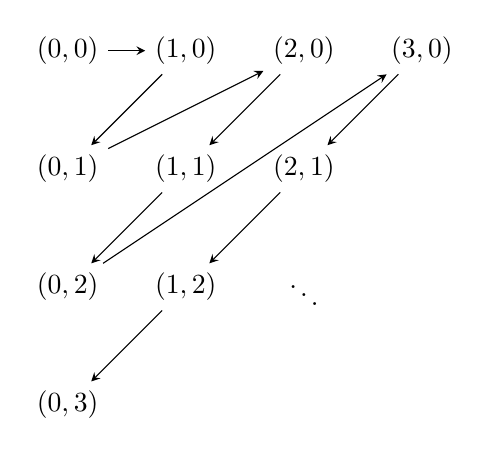
\begin{tikzpicture}[>=stealth, node distance=1.5cm]
            \node (00) {$(0, 0)$};
            \node[right of=00] (10) {$(1, 0)$};
            \node[right of=10] (20) {$(2, 0)$};
            \node[right of=20] (30) {$(3, 0)$};

            \node[below of=00] (01) {$(0, 1)$};
            \node[below of=10] (11) {$(1, 1)$};
            \node[below of=20] (21) {$(2, 1)$};
            \node[below of=01] (02) {$(0, 2)$};
            \node[below of=11] (12) {$(1, 2)$};
            \node[below of=02] (03) {$(0, 3)$};

            \node[right of=12] {$\ddots$};

            % Draw the ordering
            \draw[->] (00) edge (10) (10) edge (01) (01) edge (20) (20) edge
            (11)
            (11) edge (02) (02) edge (30) (30) edge (21) (21) edge (12) (12)
            edge (03);
        \end{tikzpicture}
        \caption{The ordering of $\N \times \N$}\label{fig:cross-ordering}
    \end{figure}
\end{proof}

\section{}
\begin{quote}
    Watch the following TED-ed talk about the Hilbert's paradox of the Grand
    Hotel.
    \begin{center}
        \url{https://www.youtube.com/watch?v=Uj3_KqkI9Zo}
    \end{center}
    Then show that the night manager could have accomplished the same result
    for the infinitely many coaches with infinitely many seats problem using
    the \textit{prime factorization method} rather than the \textit{prime
        powers method}.
\end{quote}
\end{document}
